\chapter{Introducción}\label{cap1}

\section{Anonimato en Internet}

Desde las primeras revelaciones del grupo \emph{Wikileaks}\footnote{\url{https://wikileaks.org/}} en el año 2006, 
pasando por la información revelada por el ex agente de la \emph{CIA}, \emph{Edward Snowden}\footnote{\url{http://www.huffingtonpost.com/news/nsa/}} 
en el año 2013, se ha generado un vuelco en la manera que 
los usuarios navegan por \emph{Internet}, por el hecho de tener la presunción que todos sus movimientos están siendo 
registrados por organismos de Estado, a pesar de no ser amenaza a la seguridad de las naciones que suponen proteger.

Usuarios de todo el mundo reclaman por su derecho a la privacidad\footnote{\url{http://www.livescience.com/37398-right-to-privacy.
html}}, reflejándose en tomar acciones que oculten las páginas que visitan o cualquier movimiento que realicen 
navegando en Internet a los organismos de Estado (o cualquier tercero que ellos no autoricen) que monitorean y 
recopilan dichos movimientos. Existen numerosos grupos que abogan por que se haga valer el legítimo derecho a la 
privacidad de los usuarios de Internet, argumentando sobre la importancia del anonimato\footnote{\url{https://www.derechosdigitales.org/anonimato/}} 
\footnote{\url{http://www.ted.com/talks/glenn_greenwald_why_privacy_matters}}, haciendo de éste un tema altamente 
necesario de abordar desde una perspectiva científica, brindando herramientas y protocolos que puedan asegurar el 
anonimato en Internet de manera segura, eficaz y eficiente, características centrales en el desarrollo del presente trabajo.

Hoy en dia navegar de manera anónima en Internet está vinculado fuertemente al software \emph{TOR}\footnote{\url{https://www.torproject.org/}}, 
el cual en su versión más popular se traduce en un explorador web (variante del explorador 
\emph{Firefox}\footnote{\url{https://www.mozilla.org/en-US/firefox}}) que ejecuta el protocolo \emph{onion-routing} 
(detallado en la siguiente sección), el cual permite dos objetivos: (1) ocultar la identidad del usuario tanto al proveedor 
del servicio que está consumiendo (página web que está visitando), como a algun observador externo, y (2) acceder a servicios ``ocultos'' que solo 
son accesibles con el uso de \emph{TOR}. En este trabajo nos concentraremos en el primer objetivo solamente, detallando la manera en que 
\emph{TOR} logra ocultar la identidad del usuario del servicio. Es importante nombrar que \emph{TOR} no es la única manera de 
navegar de manera anónima en Internet: \emph{I2P}\footnote{\url{https://geti2p.net/en/}} es otro servicio que provee anonimato, 
utilizar \emph{mix-networks} (explicadas a continuación) también logra ocultar la identidad del usuario, entre otros más 
detallados en este trabajo.

Anonimato, más allá del atractivo científico que posea el tema, es una cuestión socialmente difícil de abordar. Esto se debe a que 
posee contras que, puestos en un contexto determinado, pueden llegar a generar 
muchas problemáticas. Los peligros que surgen se debe a la posibilidad de realizar acciones ilícitas 
bajo el paraguas del anonimato, impidiendo su persecución. Entre estos peligros se pueden mencionar: 
denuncias falsas, compra/venta de drogas, distribución de material pornográfico infantil, fraude, \emph{bullying}, etc. 
¿Deberían los científicos crear y promover herramientas que permitan esas acciones? 
¿Valen la pena las ventajas del anonimato como para permitir la realización de estas acciones sin la posibilidad de 
perseguir a sus ejecutores?
Estas son algunas preguntas que todo científico 
debería realizarse antes de generar un trabajo (independiente del tema de investigación) que afecta directamente la sociedad en que está envuelto. 
Desde el punto de vista 
del autor, la labor del científico es siempre generar el ``mejor conocimiento'' posible, expandir la barrera del conocimiento 
humano, y al mismo tiempo, estar conciente de las posibles implicancias que posea en otras esferas de la sociedad, como por ejemplo en este caso, 
facilitar acciones ilícitas a través de Internet. 

\section{Protocolos de Anonimato}

\subsection{\emph{mix-networks}}

Una alternativa para anonimizar mensajes lo entregan protocolos de mezcla de mensajes, comúnmente llamados \emph{mixnets} 
\cite{chaum1981untraceable}, los cuáles tras un proceso de ``mezcla no invertible'', disocia datos referentes a la emisión del 
mensaje (identidad, tiempo del envío, etc.) con el mensaje mismo, impidiendo individualizar a un emisor con un mensaje en particular. 
El principal problema de este protocolo es que el anonimato se preserva gracias a una ``tercera parte confiable'' que ejecuta los 
distintos algoritmos de mezcla. Para evitar una corrupción del sistema, se utilizan varias etapas (servidores) de mezcla, dificultando 
la corrupción del sistema total (basta que un servidor sea honesto, para que todo el proceso lo sea). Sin embargo, el agregar varios servidores de 
mezcla repercute en que el proceso en su totalidad se vuelve más ineficiente, resultando en una alta latencia al momento de enviar 
un mensaje. Importante mencionar que la seguridad que se logra con este protocolo es solamente computacional (eventualmente en un futuro 
donde sea posible adquirir un mayor poder de cómputo, el sistema podría romperse).

\subsection{\emph{onion-routing}}

El protocolo más utilizado hoy en día para proveer anonimato en la red es \emph{onion-routing} 
\cite{reed1998anonymous}, utilizado principalmente a través del software \emph{TOR}. Su popularidad viene dada principalmente por 
el carácter abierto que posee el proyecto, recibiendo contribuciones por parte de voluntarios todos los 
días\footnote{\url{https://www.torproject.org/getinvolved/volunteer.html.en}}, arreglando fallas que puedan existir, además de recibir 
permanentes análisis por parte de instituciones académicas que buscan la mejora, tanto del software como del protocolo subyacente. 
Si bien el sistema posee múltiples ventajas (llegando a ser recomendado por el mismo Snowden para ocultarse de las intromisiones de 
organismos de Estado\footnote{\url{https://www.inc.com/larry-kim/5-online-privacy-tips-from-edward-snowden.html}}), 
se conocen varias falencias que posee \cite{syverson2001towards}, llegando incluso a poder romper el anonimato 
que éste provee si se posee la capacidad de monitorear toda la red (como la que poseen los distintos \emph{ISP} que proveen la conexión a 
Internet a los usuarios de la red). También es importante mencionar que el protocolo \emph{onion-routing} fue pensado bajo la amenaza 
de un adversario ``local'', es decir, que no puede monitorear toda la red. Este supuesto últimamente se ha ido debilitando, ya que 
varias filtraciones muestran que, la \emph{NSA} en particular, poseería la capacidad de monitorear todo Internet, haciendo al protocolo 
\emph{onion-routing}, y en consecuencia el software \emph{TOR}, indefensos frente a un adversario con tal poder.

\section{La Cena de Criptógrafos}

David Chaum en el año 1985 propuso un protocolo que permitía el envío de mensajes de manera anónima entre un grupo de participantes 
\cite{Chaum:1985:SWI:4372.4373, chaum1988dining}. Dicho protocolo lo ejemplificó utilizando un problema llamado ``La Cena de Criptógrafos'' 
(\emph{Dining Cryptographers Problem}), razón del porque el protocolo subsecuente sea llamado \emph{DC-Net}.

El problema, contado como una historia por su autor, es el siguiente: están 3 criptógrafos cenando tranquilamente en su restorán favorito. 
Al terminar la cena, el mozo 
se acerca a su mesa y les comunica que su cena ya está pagada y que pueden irse a sus casas. Los criptógrafos, altamente consternados, 
se miran mutuamente y llegan a la conclusión de que debió haber sucedido una de dos cosas: (1) uno de ellos pagó la cuenta de manera 
anónima (haciéndose el amable e invitando al resto sin que ellos sepan), ó (2) la cuenta fue pagada por alguien distinto a ellos 3 
(como la \emph{NSA} por ejemplo), revelando la intromisión del organismo de Estado en la vida de los criptógrafos. Es necesario poder 
dilucidar este problema, pero sin comprometer (si es que fue el caso) al criptógrafo que pagó la cuenta de manera anónima. Por lo tanto 
los criptógrafos necesitan saber si uno de ellos pagó la cuenta (sin saber quién) o si fue alguien distinto.

David Chaum generaliza el problema de la siguiente manera: se tienen 3 participantes (los criptógrafos) donde cada uno de ellos quiere 
comunicar un mensaje (pagó o no pagó la cena). El resultado del protocolo debe entregar, ya sea el mensaje de alguno de ellos 
(que pagó la cena), sin conocer el emisor de dicho mensaje, o bien que todos los mensajes fueron iguales (revelando que nadie pagó la cena, concluyendo 
que fue un agente externo). El protocolo debe mantener el anonimato del participante que envió el mensaje tanto para el resto de los 
participantes como para cualquier observador externo que esté monitoreando las conversaciones.

La solución propuesta supone el envío de solo 1 bit de información (en el caso del problema, pagó o no pagó la cena). 
La solución generalizada consiste en los siguientes pasos:
\begin{enumerate}
    \item Cada par de participantes $(p_i, p_j)$ escogen un bit al azar compartido $b_{ij}$.
    \item Cada participante $p_i$ calcula $b_i$ como la operación $\oplus$\footnote{La operación $\oplus$ (\texttt{XOR}) entre 
    dos bits, entrega 1 como resultado si y solo si ambos bits son distintos, 0 si son iguales.} entre todos los $b_{ij}$ que posea 
    compartidos. Por ejemplo, en el caso de la cena: $b_1 = b_{12} \oplus b_{13}$, $b_2 = b_{12} \oplus b_{23}$, $b_3 = b_{13} \oplus b_{23}$.
    \item Cada participante $p_i$ define su propio $M_i$, el cual corresponderá al bit que quiere comunicar ($M_i = 1$ si pagó la cena).
    \item Cada $p_i$ revelará el valor $o_i = M_i \oplus b_i$.
    \item Cualquier $p_i$ u observador externo puede calcular el valor $D = \displaystyle\bigoplus_i o_i$.
    \item Si $D = 1$, entonces uno de los participantes envió el mensaje 1 (alguien pagó la cena), si $D = 0$, todos los participantes 
    enviaron el mensaje 0 (la cena la pagó un agente externo a los participantes).
\end{enumerate}

\begin{figure}[H]
\centering
\subfigure[Compartición de bit al azar $b_{ij}$ entre cada par de participantes.] { \begin{footnotesize}
\newcommand{\participK}[2]{
\begin{scope}[shift={(#1)}]
\draw [draw,fill=lightgray] (0pt,10pt) circle (5pt);
\draw [draw,fill=lightgray] (10pt,0pt) arc (0:180:10pt and 5pt);
\fill [lightgray] (-10pt,-10pt) rectangle (10pt,0pt);
\draw [draw] (10pt,0pt) -- (10pt,-10pt);
\draw [draw] (-10pt,0pt) -- (-10pt,-10pt);
\draw [draw] (5pt,-1pt) -- (5pt,-10pt);
\draw [draw] (-5pt,-1pt) -- (-5pt,-10pt);
\draw [anchor=center] (0pt,-2.5pt) node {#2};
\end{scope}
}
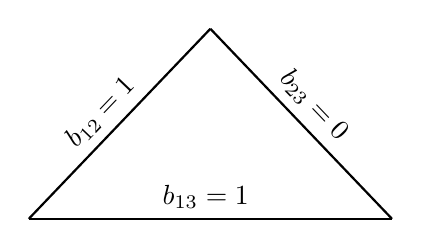
\begin{tikzpicture}
\begin{scope}
\path (18:6.9em) coordinate (P3);
\path (90:9em) coordinate (P2);
\path (162:6.9em) coordinate (P1);
\draw [thick] (P3) to node [anchor=south ,pos=0.5,swap,sloped] {$b_{23} = 0\ $} (P2);
\draw [thick] (P3) to node [anchor=south ,pos=0.5,swap,sloped] {$b_{13} = 1\ $} (P1);
\draw [thick] (P2) to node [anchor=south ,pos=0.5,swap,sloped] {$b_{12} = 1\ $} (P1);

\participK{P1}{$P_1$};
\participK{P2}{$P_2$};
\participK{P3}{$P_3$};
\end{scope}


\end{tikzpicture}
\end{footnotesize}\label{2a} } \  
\subfigure[Cálculo de $o_i$ por cada participante, dependiendo si pagó o no la cena.] { \begin{footnotesize}
\newcommand{\participK}[2]{
\begin{scope}[shift={(#1)}]
\draw [draw,fill=lightgray] (0pt,10pt) circle (5pt);
\draw [draw,fill=lightgray] (10pt,0pt) arc (0:180:10pt and 5pt);
\fill [lightgray] (-10pt,-10pt) rectangle (10pt,0pt);
\draw [draw] (10pt,0pt) -- (10pt,-10pt);
\draw [draw] (-10pt,0pt) -- (-10pt,-10pt);
\draw [draw] (5pt,-1pt) -- (5pt,-10pt);
\draw [draw] (-5pt,-1pt) -- (-5pt,-10pt);
\draw [anchor=center] (0pt,-2.5pt) node {#2};
\end{scope}
}
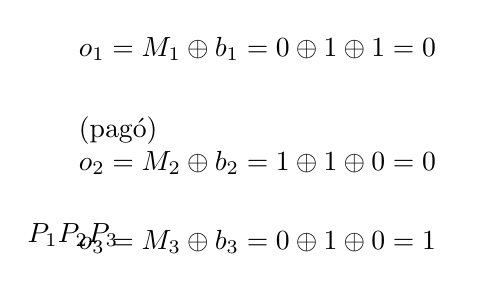
\begin{tikzpicture}

\begin{scope}
\path (0em,7em) coordinate (Q1);
\path (0em,3.5em) coordinate (Q2);
\path (0em,0em) coordinate (Q3);

\node [rectangle, right of=Q1, anchor=west, node distance=1.5em] {$o_1 = M_1 \oplus b_1 = 0 \oplus 1 \oplus 1 = 0$};
\node [rectangle, right of=Q2, anchor=west, node distance=1.5em, text width=136pt] {(pagó)\\$o_2= M_2 \oplus b_2 = 1 \oplus 1 \oplus 0 = 0$};
\node [rectangle, right of=Q3, anchor=west, node distance=1.5em] {$o_3= M_3 \oplus b_3 = 0 \oplus 1 \oplus 0 = 1$};

\participK{Q1}{$P_1$};
\participK{Q2}{$P_2$};
\participK{Q3}{$P_3$};
\end{scope}

\end{tikzpicture}
\end{footnotesize}
\label{2b} }

\protect\caption{Ejemplo de Cena de Criptógrafos donde uno de los participantes pagó la cena. En este caso $D = 0 \oplus 0 \oplus 1 = 1$. 
No es difícil observar que si ningún participante pagó la cena, $D = 0$. }

\label{fig:example_dcnet_chaum}
\end{figure}

Luego de proponer esta solución, David Chaum realiza el análisis de seguridad del protocolo (para más detalles consultar el paper original 
\cite{chaum1988dining}), del cual concluye que el protocolo sugerido entrega anonimato de manera \emph{incondicional}, es decir, que incluso 
un adversario que posea todo el poder de cómputo posible no puede dar con una estrategia que le permita encontrar al emisor del mensaje 
con mejor probabilidad que $1/n$ (donde $n$ es la cantidad total de participantes).

Posteriormente se propone una manera de generalizar el protocolo para utilizarlo con mensajes más largos (de más de 1 bit), lo cual será 
visto en la siguiente sección.

\section{\emph{DC-Net} como protocolo de anonimato}

\emph{DC-Net} (\emph{Dining Cryptographers Network}) es un protocolo que permite enviar un mensaje de manera anónima a un grupo de participantes 
(llamado \emph{anonimity-set}), el cual protege la identidad del emisor (que debe ser parte del \emph{anonimity-set}) del mensaje de manera 
\emph{incondicional}, es decir, que cualquier adversario (independiente del poder de cómputo que posea) no puede encontrar a dicho emisor con 
una probabilidad mayor a $1/n$ (donde $n$ es el tamaño del \emph{anonimity-set} o la cantidad total de participantes). Dicho adversario puede 
ser interno (ser uno de los participantes) o externo (que puede estar potencialmente monitoreando todas las comunicaciones entre los distintos participantes).

A continuación se detallará la generalización del protocolo para permitir el envío de mensajes de largo arbitrario. 
Supongamos un \emph{anonimity-set} de $n$ participantes $\{p_1, p_2, \ldots, p_n\}$. Sin perdida de generalidad, supondremos que $p_1$ es el único 
participante que quiere enviar un mensaje (más adelante 
se hablará cuando dos o más participantes quieren enviar un mensaje), 
en este caso $M_1 = m \in \mathbb{Z}_q$\footnote{$\mathbb{Z}_q = \{1, 2, \ldots, q - 1\}$}, para todo el resto $M_i = 0$ $(\forall i \in \{2, \ldots, n\})$.

El primer paso, al igual que en el protocolo original, es generar valores (llaves) compartidos entre cada par de participantes. Con esto 
tendremos que cada par $\{p_i, p_j\}$ compartirá un valor único $k_{ij}$ (además se definirá que $k_{ij} = -k_{ji}$ y $k_{ii} = 0$).

\begin{figure}[H]
  \centering
    \includegraphics[width=0.5\textwidth]{imagenes/dcnet-general-03.png}
  \caption{Llaves compartidas en DC-Net}
\end{figure}

Con esto, cada participante $p_i$ generará un valor igual a la suma de todas las llaves compartidas que posee, esto es $K_i = \sum_{j=1}^n k_{ij}$. 
Luego, deberá generar el valor que comunicará al resto de los participantes, que consistirá en la suma del valor $K_i$ con el mensaje $M_i$, 
generando $O_i = K_i + M_i$ (recordemos que solo $p_1$ posee su mensaje distinto a 0, por lo que para el todo el resto de los participantes $O_i = K_i$). 
Finalmente, cada participante enviará el valor $O_i$ al resto de los participantes (mensaje vía \emph{broadcast}, por ejemplo). Con esto, los 
valores $O_i$ quedan disponibles tanto para el resto de los participantes, como para cualquier observador externo.

Ahora solo queda encontrar el mensaje enviado por $p_1$. Para ello, se calcula el valor $D$ como la suma de todos los $O_i$ enviados por los 
participantes: $$D = \sum_{i=1}^n O_i \overset{(1)}{=} \sum_{i=1}^n K_i + \sum_{i=1}^n M_i \overset{(2)}{=} \sum_{i=1}^n K_i + m \overset{(3)}{=} m$$

La primera (1) simplificación se debe a la definición de $O_i$ y la separación de la suma en las dos componentes $K_i$ y $M_i$. La segunda 
(2) hace referencia al hecho que $M_i = 0$ $\forall i \geq 2$, por lo que solo ``sobrevive'' $M_1 = m$. Finalmente la tercera (3) simplificación 
se debe al hecho que las llaves compartidas se cancelan mutuamente, debido al hecho que se explicitó que $k_{ij} = -k_{ji}$. Por lo tanto, el 
valor $D$ corresponde al único mensaje enviado $m$, revelando su valor al resto de los participantes, y manteniendo en el anonimato a su emisor 
(en este caso, $p_1$).

Informalmente, se puede decir que el mensaje $m$ se oculta entre la suma de las llaves compartidas, que junto con la imposibilidad de conocer el 
valor de todas las llaves compartidas (a menos que se coludan $n-1$ participantes), es imposible poder dilucidar si un mensaje $m$ vino de un 
cierto $O_i$ revelado por algún participante.

Ahora bien, el protocolo anteriormente descrito sufre de dos problemas: (1) el protocolo funciona sólo cuando un 
único participante envía un mensaje, de haber dos o más participantes con $M_i \neq 0$, se tendría que $D = \sum M_i$, por lo que sería imposible 
rescatar los mensajes individuales. Por otro lado, (2) no evita que participantes maliciosos envíen mensajes erróneos, por ejemplo, que envíen 
valores de llaves compartidas distintos, haciendo que estos no se cancelen, imposibilitando la revelación del mensaje $m$ final. Es por ello que 
las distintas variantes del protocolo que se propongan, deben tener como prioridad soslayar estos dos problemas inherentes al protocolo. En este 
trabajo se detallará una variante que soluciona estos problema utilizando herramientas criptográficas que serán presentadas en el próximo capítulo.

\section{Objetivos del Trabajo}

\subsection{Objetivo General}

Diseñar e implementar una variante del protocolo \emph{DC-Net} que alcance niveles de seguridad tales que mejoren los ofrecidos por otros protocolos 
actualmente utilizados para mantener anonimato. Además de encontrar escenarios donde la implementación presente mejores resultados que las 
alternativas existentes, tomando en cuenta distintos factores como lo son la seguridad alcanzada y el tiempo de ejecución necesario para el envío de los mensajes.

\subsection{Objetivos Específicos}

\begin{itemize}
    \item Analizar las actuales soluciones (protocolos) que brindan anonimato con el fin de encontrar aspectos que puedan ser mejorados en la propuesta 
    final del presente trabajo.
    \item Encontrar otras implementaciones de variantes de \emph{DC-Net}, identificando aspectos a mejorar, además de poder disminuir los supuestos de 
    seguridad en que se basan dichas soluciones.
    \item Poner a prueba la implementación realizada en distintos escenarios, analizando el tiempo de ejecución en cada uno de ellos, con el objetivo 
    de encontrar el mejor contexto en que se desempeñaría la solución final.
    \item Crear un caso de prueba del sistema implementado, que sirva como motivación a distintos posibles usos que se le pueda dar al código realizado.
\end{itemize}

\section{Organización del Documento}

En el presente documento se describen los pasos que se siguieron para la propuesta de un diseño y una implementación de un sistema de mensajería que 
provee anonimato a los emisores, todo ello basado en el protocolo \emph{DC-Net}. En el Capítulo \ref{cap2} se describen los antecedentes criptográficos 
necesarios para comprender la solución propesta, además de un análisis de soluciones similares propuestas en otros trabajos. Luego en el Capítulo \ref{cap3} 
se describe de manera detallada el diseño de la variante propuesta, especificando paso a paso lo que cada uno de los participantes debe realizar 
para poder contar con el sistema que se propuso como objetivo. Posteriormente en el Capítulo \ref{cap4} se presentan detalles de la implementación del diseño 
descrito anteriormente, exponiendo decisiones que se fueron tomando para la conformación del sistema finalmente implementado (además de una breve 
descripción de un caso de uso, en este caso, una aplicación móvil). En el Capítulo \ref{cap5} se detallan los experimentos que se llevaron a cabo para probar, 
sobre todo, el tiempo de ejecución del sistema, exponiéndolo a distintos escenarios y obteniendo distintos resultados que son discutidos en la parte 
final del capítulo. Luego en el Capítulo \ref{cap6} se 
brindan posibles mejoras que se le puedan hacer tanto al protocolo diseñado como a la implementación realizada. Finalmente en el Capítulo \ref{cap7} se 
presentan tanto las conclusiones del presente trabajo, como las experiencias que dejaron tanto su diseño como su implementación.
